\section{Results}

\subsection{Existence Verification (RQ1)}

\begin{table}[h]
\centering
\caption{h-e1-v2 Existence Verification Results.}
\label{tab:verification}
\begin{tabular}{lllll}
\toprule
Condition & Metric & Target & Actual & Status \\
\midrule
C1: Failure IDs & Total failures & 134 & 134 & PASS \\
C1: Failure IDs & HumanEval$+$ & 34 & 34 & PASS \\
C1: Failure IDs & MBPP$+$ & 100 & 100 & PASS \\
C2: Stored solutions & Cache coverage & 134/134 & 134/134 & PASS \\
C3: EvalPlus API & HE$+$ accessible & 34/34 & 34/34 & PASS \\
C3: EvalPlus API & MBPP$+$ accessible & 100/100 & 100/100 & PASS \\
C4: Test selection & \texttt{plus\_input} count & $>$ 0 & 780 & PASS \\
\bottomrule
\end{tabular}
\end{table}

All 5 pytest tests pass in 2.32 seconds. The 4/4 condition pass rate confirms that
Conditions B and C prompts can be constructed for 128 tasks without new baseline
API calls.

\subsection{Static Analysis Oracle Falsification}

\begin{table}[h]
\centering
\caption{Static Analysis Fire Rates on EvalPlus Failures (h-e1 Run 2).}
\label{tab:sa-rates}
\begin{tabular}{lll}
\toprule
Benchmark & SA fire rate & Problems with no SA signal \\
\midrule
HumanEval$+$ (n$=$34) & 32.4\% & 67.6\% (23/34) \\
MBPP$+$ (n$=$100) & 16.0\% & 84.0\% (84/100) \\
\bottomrule
\end{tabular}
\end{table}

These rates establish the motivation for specification-aligned repair: two-thirds to
five-sixths of failures receive no actionable SA feedback.

\subsection{Data Integrity Finding}

\begin{figure}[t]
\centering
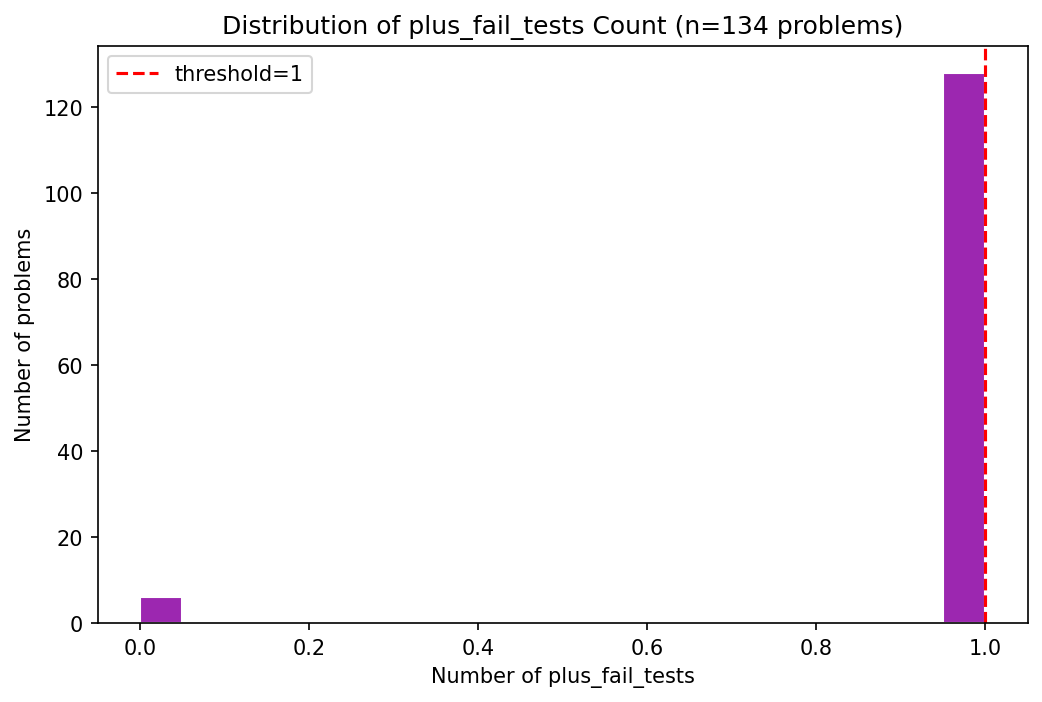
\includegraphics[width=0.75\textwidth]{figures/failing_tests_histogram.png}
\caption{Histogram of \texttt{plus\_fail\_tests} count per problem in the h-e1 archive. Six problems (HumanEval/143, Mbpp/725, 726, 765, 805, 809) have empty failing-test fields, yielding a 128-problem working set for Conditions B and C.}
\label{fig:failing-tests-histogram}
\end{figure}

Figure~\ref{fig:failing-tests-histogram} shows that 6/134 archive records have \texttt{plus\_fail\_tests = []} despite
\texttt{plus\_status = ``fail''}. The most likely cause is test runner timeout during h-e1
Run 2. Figure~\ref{fig:completeness-matrix} (completeness heatmap) shows these as isolated white cells --- a
localized data gap, not a systematic failure. The 128-task working set (95.5\%
recovery) is the appropriate scope for mechanism experiments.

\begin{figure}[t]
\centering
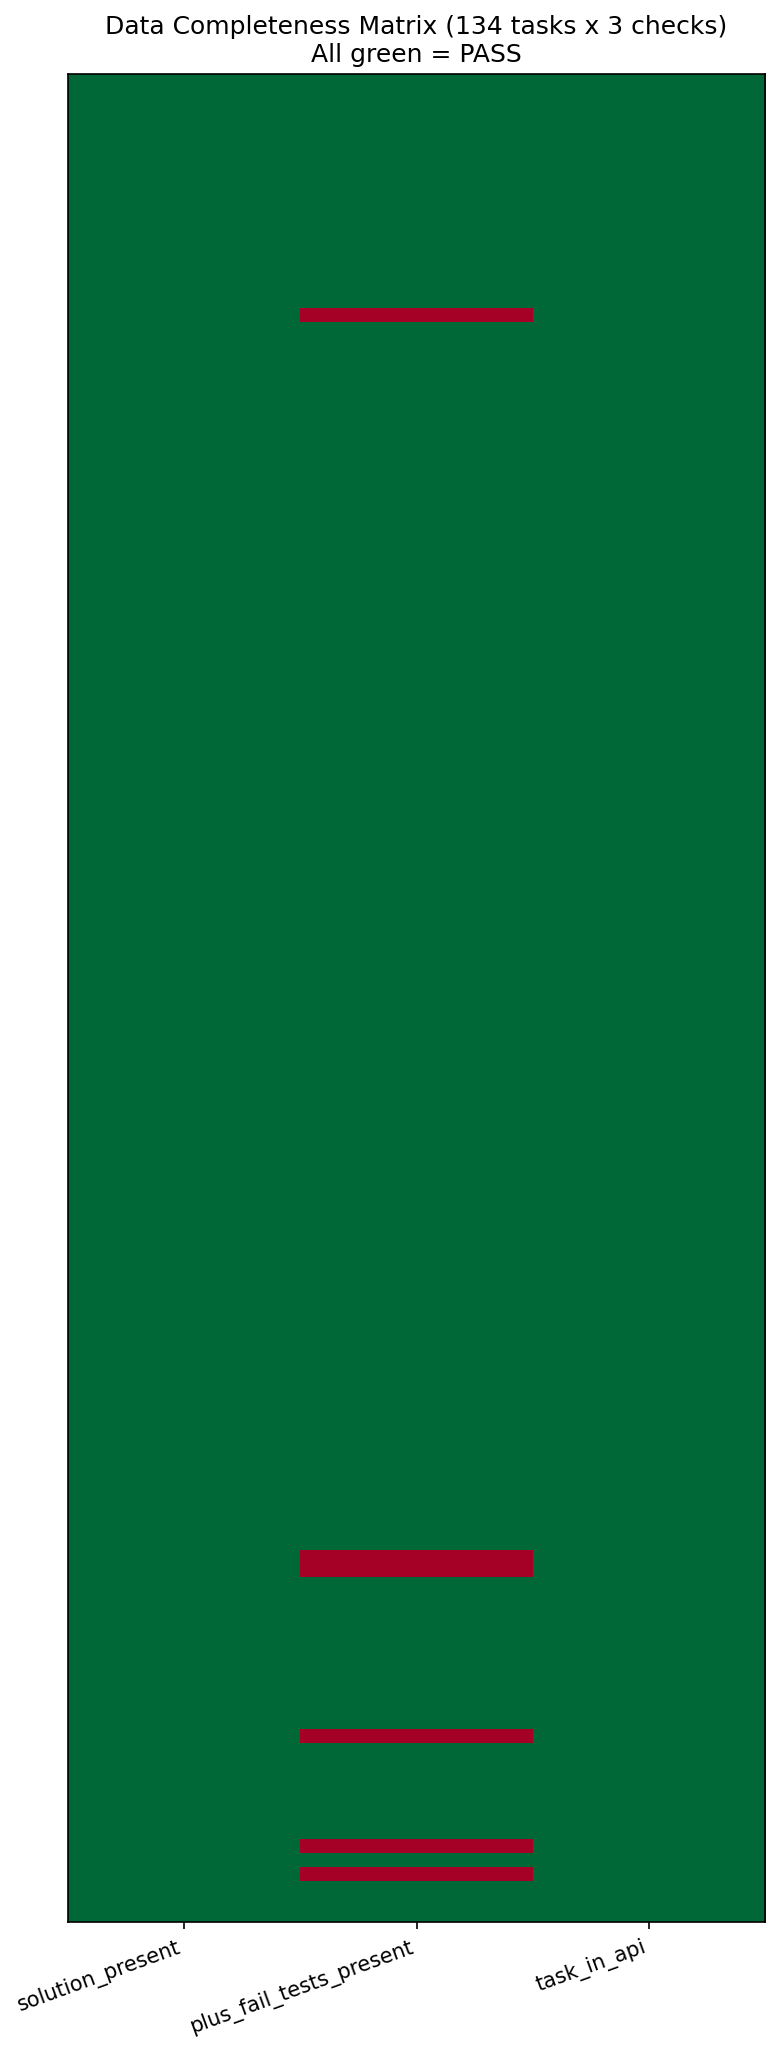
\includegraphics[width=0.85\textwidth]{figures/completeness_matrix.png}
\caption{Completeness heatmap for all 134 failure records across three fields (solution, \texttt{plus\_fail\_tests}, \texttt{plus\_status}). Six records show missing \texttt{plus\_fail\_tests} (white cells), confirming the 128/134 recovery rate.}
\label{fig:completeness-matrix}
\end{figure}

This finding also validates the h-e1 $\rightarrow$ h-e1-v2 redesign decision: \texttt{solutions\_cache.jsonl}
(134/134 complete) is the correct data source for Condition B/C prompt construction,
not the archived \texttt{plus\_fail\_tests} (which has 6 gaps).

\subsection{Pre-Registered Predictions}

\begin{table}[h]
\centering
\caption{Pre-Registered Prediction Status.}
\label{tab:predictions}
\begin{tabular}{lllll}
\toprule
Prediction & Statement & Test & Target & Status \\
\midrule
P1 & C $>$ B (McNemar, one-tailed) & h-m1 & p $<$ 0.05 & INCONCLUSIVE \\
P2 & C $>$ A (fix rate $\geq$ 15\%) & h-m2 & p $<$ 0.05, $\geq$15\% & INCONCLUSIVE \\
P3 & HE$+$ fix rate $>$ MBPP$+$ fix rate & h-c1 & Directional & INCONCLUSIVE \\
\bottomrule
\end{tabular}
\end{table}

INCONCLUSIVE indicates predictions registered before data collection; the existence
gate PASS unblocks all three mechanism experiments.

\subsection{Statistical Power for Planned Experiments}

At n$=$128, expected scenario (25\% fix rate under C, 10\% under B): $\sim$24 discordant
pairs, McNemar power $\sim$80\% at $\alpha=$0.05 one-tailed. Adequate for pre-registered predictions.
